\setlength{\columnsep}{3pt}
\begin{flushleft}
	
	\begin{itemize}
		\item An IP address is a \textbf{unique address that identifies a device} on the internet or a local network.
		\item Command to check IP address:
		\bigskip
		\begin{tcolorbox}[breakable,notitle,boxrule=-0pt,colback=pink,colframe=pink]
			\color{black}
			\fontdimen2\font=1em
			Syntax: ifconfig
			\newline
			or
			\newline
			Syntax: ip addr
			\fontdimen2\font=4pt
		\end{tcolorbox}
		\item Eg:
		\begin{figure}[h!]
			\centering
			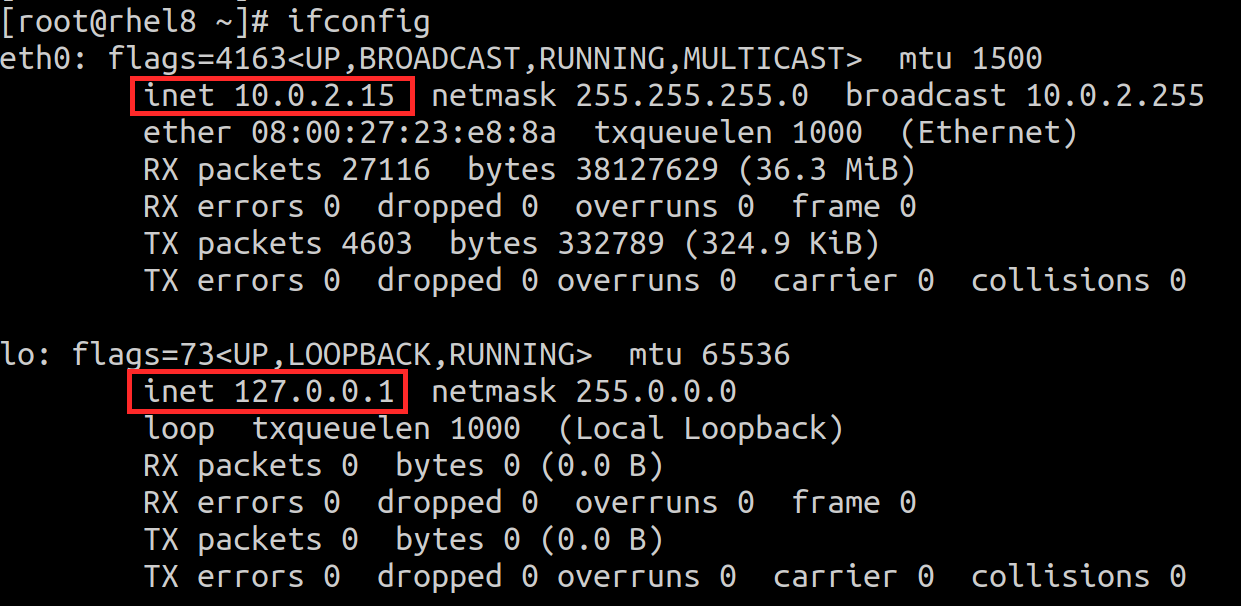
\includegraphics[scale=.25]{content/chapter14/images/ifconfig.png}
			\caption{Sample output}
			\label{fig:ifconfig}
		\end{figure}	
		
	\end{itemize}
		
\end{flushleft}
\newpage


